\documentclass[12pt]{article}
%\usepackage[margin=1in]{geometry}
\usepackage[a4paper, width=150mm, top=25mm, bottom=25mm]{geometry}

%link
\usepackage{amsfonts, amsmath, amssymb}
\usepackage{hyperref}
\usepackage{url}

\usepackage{color}
\newcommand{\Color}[1]{%
    \pdfcolorstack\pdfcolorstackinit page direct{0 g}%
     push {#1 rg}%
}

\usepackage{}
%table-image
\usepackage{graphicx}
\usepackage{float}

%\usepackage[nottoc, notlot, notlof]{tocbibind}
\parindent 0ex
%\setlength{\parindent}{4em}
%\setlength{\parskip}{1em}  %spacce btw paragraphs
\renewcommand{\baselinestretch}{1.5}{}
{}
%-
\begin{document}
\begin{titlepage}
\begin{center}
\vspace{1cm}
\large{\textbf{RESEARCH PROPOSAL}}
\line(1,0){400}\\
\vfill

\line(1,0){400}\\[1mm]
\huge{\textbf{Research Title}}\\[1mm]
\large{\textbf{- This is a Sample Title -}}\\[1mm]
\line(1,0){400}\\[1mm]
\vfill

By NAME\\
Candidate N0\\
\vfill

Dr. NAME\\
Dr. NAME\\
Dr. NAME\\

\today\\
\end{center}
\end{titlepage}

\tableofcontents
\thispagestyle{empty}
\clearpage

\setcounter{page}{1}
\section{Introduction}

\section{Abstract}

\section{Objectives}
"Provide a clearly defined statement of the objectives of the research." Sometimes only one objective; sometimes one board AIM, and several objectives.\\
Use active verbs, i.e. propose, create, construct, demonstrate, define, establish, differentiate.
\section{Background}
\subsection{Method 1}
\subsection{Method 2}
\subsection{Method 3}
\subsection{Method 4}
\section{Significance}
\section{Research Method}

% \begin{tabular}{|c|c|}
% \hline%
%     \LCC%
%         \Color{0 0 1}& \Color{1 1 0}\\ % "Fake" row with color definitions
%         Blue & Yellow \\
%     \ECC\hline
%     Normal & Normal\\ \hline
% \end{tabular}

\section{Ethical Issues}
\section{Facilities \& Resources}
\section{Data Storage}
\section{Time Line}


\newpage
Sample file: Links on the class website \url{http://prancer.physics.louisville.edu/classes/308/} \\
Figure \ref{fig:graph1} is an example of  how to do it in \LaTeX \footnote{An example of footnotes}.\\
\begin{figure}[h]  %t: top, h:exact position
	\begin{center}
	\resizebox{4in}{!}{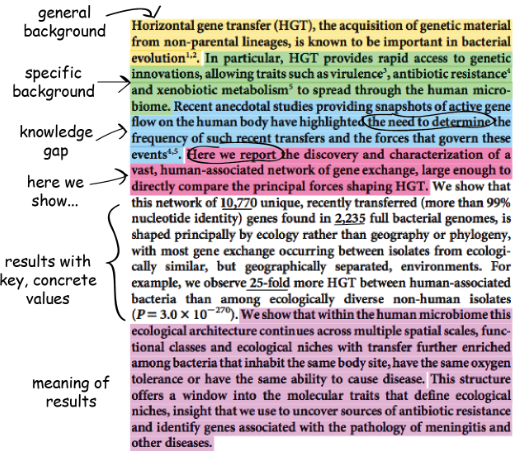
\includegraphics{good_abstract.png}}{}
	\end{center}
	\caption{The Orion Nebula, M42, recorded with the CDK20N telescope on the night of November 1, 2011.}
	\label{fig:graph1}
\end{figure}

The paper \cite{cole1989kinematics} and \cite{sadeghi2009review} showed that ,,,,
\newpage
\bibliographystyle{ieeetr}
\bibliography{citation}

\end{document}
